\documentclass[tikz,border=10pt]{standalone}
% Only base TikZ is needed
\begin{document}
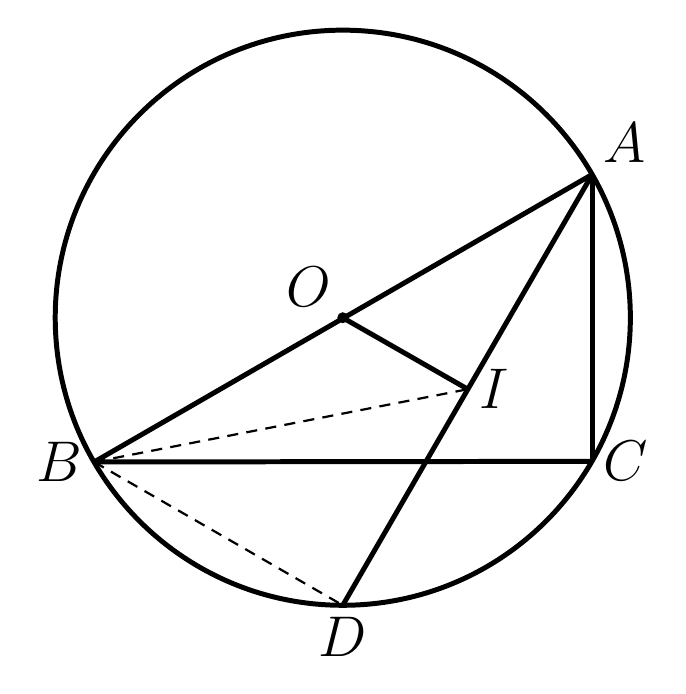
\begin{tikzpicture}[line width=1.8pt, line join=round]
  % Named coordinates (cm), s = 0.015474 units per px, y flipped
  \coordinate (O) at (0,0);
  \coordinate (A) at (3.168,1.820);
  \coordinate (B) at (-3.157,-1.832);
  \coordinate (C) at (3.168,-1.824);
  \coordinate (D) at (0,-3.652);
  \coordinate (I) at (1.588,-0.908);
  \coordinate (P) at (1.054,-1.832);  % unlabeled point on BC (not labelled)

  % Circle centred at O, radius 236 px
  \draw (O) circle (3.652);

  % Solid segments
  \draw (B) -- (A);     % diameter through O
  \draw (B) -- (C);     % horizontal
  \draw (A) -- (C);     % vertical
  \draw (A) -- (D);     % passes through P
  \draw (O) -- (I);

  % Dashed segments: thin, explicit dash pattern
  \draw[line width=0.8pt, dash pattern=on 4pt off 3pt] (B) -- (I);
  \draw[line width=0.8pt, dash pattern=on 4pt off 3pt] (B) -- (D);

  % Dot at O
  \fill (O) circle (0.07);

  % Labels (larger math-italic, ~22pt)
  \node[above right, font=\fontsize{22}{26}\selectfont] at (A) {$A$};
  \node[left, font=\fontsize{22}{26}\selectfont] at (B) {$B$};
  \node[right, font=\fontsize{22}{26}\selectfont] at (C) {$C$};
  \node[below, font=\fontsize{22}{26}\selectfont] at (D) {$D$};
  \node[above left, font=\fontsize{22}{26}\selectfont] at (O) {$O$};
  \node[right, font=\fontsize{22}{26}\selectfont] at (I) {$I$};
\end{tikzpicture}
\end{document}